\documentclass[12pt]{article}
\usepackage[english]{babel}
\usepackage[utf8x]{inputenc}
\usepackage[T1]{fontenc}
\usepackage{listings}
\usepackage{bookmark}
\usepackage{tikz}
\makeatletter
\def\input@path{{../../style/}}
\makeatother

\usepackage{../../style/quiver}
\makeatletter
\def\input@path{{../../style/}}
\makeatother

\usepackage{../../style/scribe}
\usepackage{fancyhdr}

\usepackage{parskip} % Automatically respects blank lines
\usepackage{booktabs} % For \addlinespace command
\setlength{\parskip}{1em} % Adds more space between paragraphs
\setlength{\parindent}{0pt} % Removes paragraph indentation

\begin{document}


\lhead{Songyu Ye}
\rhead{\today}
\cfoot{\thepage}

\title{Autoequivalences from GIT}

\author{Songyu Ye}
\date{\today}
\maketitle


\begin{abstract}
Notes for a talk on autoequivalences arising from variation of GIT quotients, given in the low dimensional gauge theory seminar at UC Berkeley. 
\end{abstract}

\tableofcontents

\section{Motivation}
Homological mirror symmetry predicts that in certain cases,
derived categories of coherent sheaves on an algebraic variety should admit twist autoequivalences corresponding to a spherical object.
\begin{enumerate}
    \item A-model: symplectic automorphisms and generalized Dehn twists along Lagrangian spheres
    \item B-model: derived autoequivalences such as spherical twists
\end{enumerate}
We want to consider natural constructions of twist autoequivalences of $D^b(X)$. Techniques come from variation of GIT (VGIT) and the general theory of spherical functors and semiorthogonal decompositions.

\section{Refresher on GIT}
Consider a graded noetherian algebra over $\C$:
\[
R = \bigoplus_{m=0}^\infty R_m
\] 
The variety $X = \Proj R$ is projective over the affine variety $\Spec R_0$, and comes equipped with an ample line bundle $\cL = \O_X(1)$.  

Let $G$ be a reductive algebraic group acting on $R$ by graded algebra automorphisms. Then $G$ acts on $X$ and $\cL$ is a $G$-linearized ample line bundle.  We can form the GIT quotient
\[
X /\!/ G := \Proj(R^G)
\]
The invariant algerbra is finitely generated (Hilbert, Nagata).

The inclusion $R^G \subset R$ induces a rational map
\[
X \dashrightarrow X /\!/ G.
\] 
\begin{definition}
    A point $x \in X$ is semistable if it is in the domain of definition of the above rational map. A point $x \in X$ is stable if its orbit is closed in the semistable locus and its stabilizer is finite. Denote the semistable locus by $X^{ss}$ and the stable locus by $X^s$.
\end{definition}
The map $X^{ss} \to X /\!/ G$ is the GIT quotient.

\subsection{Chambers}
Fix an ample line bundle $L$ on $X$. The space of G-linearizations of $L$ has a wall-chamber structure; crossing a wall changes the GIT quotient by a birational map.

\begin{theorem}
    The real character space $X^\ast(G)_\R$ is cut into finitely many chambers by rational walls; for characters in the same chamber the GIT quotient $X^{ss}(L,\chi) \to X /\!/_{L,\chi} G$
     is constant, and crossing a wall induces a birational modification of the quotient.
\end{theorem}

It is also true that there are only finitely many distinct GIT quotients
$X /\!/_{L} G$ up to isomorphism as $L$ ranges over all $G$--ample
linearizations.

Restriction gives an exact dg-functor $i^\ast: D^b(X/G) \to D^b(X^{ss}/G)$. One important fact that we will see later is that there is a functorial splitting.

\section{The standard flop}
We do an example following Segal. Let $V = \mathbb{C}^4_{x_1,x_2,y_1,y_2}$ and $\mathbb{C}^*$ act on $V$ with weight $(1,1,-1,-1)$.

There are two possible GIT quotients $X_{+}$ and $X_{-}$, depending on whether we choose a positive or negative character of $\mathbb{C}^*$. Both are isomorphic to the total space of the bundle $\mathcal{O}(-1)^{\oplus 2}$ over $\mathbb{P}^1$.

Open substacks of the stack $\mathcal{X} = [V/\mathbb{C}^*]$ given by the semistable loci. Let $\iota_\pm: X_\pm \to \mathcal{X}$ be the open immersions. The restriction functors $\iota_\pm^*: D^b(\mathcal{X}) \to D^b(X_\pm)$ are exact.

Let $\cG_t = \langle \cO(t), \cO(t+1) \rangle \subset D^b(\mathcal{X})$. It is called a window subcategory.

\begin{claim}
For any $t \in \mathbb{Z}$, both $\iota_+^*$ and $\iota_-^*$ restrict to give equivalences
  \[
    D^b(X_+) \xleftarrow{\sim} \mathcal{G}_t \xrightarrow{\sim} D^b(X_-).
  \]
\end{claim}

\begin{proof}
    Exactness, preserves shifts and cones, are clear. 
    To check fully faithfulness, it is enough to show that $H^\bullet_{\mathcal{X}}(\mathcal{O}(i)) = H^\bullet_{X_\pm}(\mathcal{O}(i))$ for $i \in [-1,1]$.

Left hand side: $V$ affine, so $H^p(\mathcal{X},\mathcal{O}(i))=(\mathcal{O}_V)_i$ for $p=0$ and $0$ for $p>0$. 

Right hand side: We do the computation for $X^+$. Let projection $\pi:X_+ \to\mathbb{P}^1$. Recall $X_+$ is the total space of the bundle $E = \mathcal{O}(-1)^{\oplus 2}$ over $\mathbb{P}^1_x$. 

By the projection formula and affineness of $\pi$ \[
  H^p(X^+,\mathcal{O}_{X_+}(k))
  \cong
  H^p\Big(\mathbb{P}^1,\ \pi_*\mathcal{O}_{X^+}\otimes\mathcal{O}(k)\Big)
  \cong
  \bigoplus_{m\ge0} H^p(\mathbb{P}^1,\ \mathcal{O}(k+m))^{\oplus (m+1)}
\]
When $p=0$, this has global sections \begin{align*}
\Sym^{k+m}(\mathbb C^2_{x_1,x_2}) \otimes \Sym^m(\mathbb C^2_{y_1,y_2})
\end{align*}
which is exactly the degree $k$ piece of $\mathcal{O}_V$. When $p>0$, this is zero for $k=-1,0,1$.

For $p=1$, recall $k \in {-1,0,1}$ and $m\ge0$, so $k+m\ge -1$. Thus $H^1(\mathbb{P}^1,\ \mathcal{O}(k+m))=0$. This agrees with the left hand side. Note that if the size of the window is bigger, then we would pick up some $H^1$ terms.

Essential surjectivity follows from exactness of \[\pi^*: \Coh(\P^1) \to \Coh(X_\pm)\] and the fact that $D^b(\P^1)$ is generated by $\cO_{\P^1}(t), \cO_{\P^1}(t+1)$ by Beilinson's theorem.
\end{proof}

So for any $t\in\mathbb{Z}$ we have a derived equivalence
\[
  \Phi_t : D^b(X_+) \;\xrightarrow{\ \sim\ }\; D^b(X_-)
\]
passing through $\mathcal{G}_t$. Composing these, we get auto-equivalences
\[
  \Phi_{t+1}^{-1}\Phi_t : D^b(X_+) \;\xrightarrow{\ \sim\ }\; D^b(X_+).
\]
To see what these do, we need to check them on the generating set of line-bundles
$\{\mathcal{O}(t), \mathcal{O}(t+1)\}$. 

Consider the Koszul resolution resolving the structure sheaf of the unstable locus $\{y_1=y_2=0\}$:
\[
  0 \to \mathcal{O}_V(2) \xrightarrow{(y_2,-y_1)} \mathcal{O}_V(1)^{\oplus 2} \xrightarrow{(y_1,y_2)} \mathcal{O}_V \to \cO_V/\{y_1=y_2=0\} \to 0
\]

Restricting the sequence to $X^-$, the resolution becomes exact at the end since the unstable locus $\{y_1=y_2=0\}$ is removed in $X^-$. Thus on $X^-$ we have a quasi-isomorphism:
\[
  \mathcal{O}_{X^-}(k) \simeq \big[ \mathcal{O}_{X^-}(k+2) \xrightarrow{(y_2,-y_1)} \mathcal{O}_{X^-}(k+1)^{\oplus 2} \big]
\] 
Thus we compute:
\begin{align*}
  \Phi_{t+1}^{-1}\Phi_t(\mathcal{O}_{X_+}(t))
  &\simeq \Phi_{t+1}^{-1}(\mathcal{O}_{X_-}(t)) \\
  &\simeq \Phi_{t+1}^{-1}\Big(\big[\mathcal{O}_{X_-}(t+2) \xrightarrow{(y_2,-y_1)} \mathcal{O}_{X_-}(t+1)^{\oplus 2}\big]\Big) \\
  &\simeq \big[\mathcal{O}_{X_+}(t+2) \xrightarrow{(y_2,-y_1)} \mathcal{O}_{X_+}(t+1)^{\oplus 2}\big], \\
  \Phi_{t+1}^{-1}\Phi_t(\mathcal{O}_{X_+}(t+1))
  &\simeq \Phi_{t+1}^{-1}(\mathcal{O}_{X_-}(t+1)) \\
  &\simeq \mathcal{O}_{X_+}(t+1).
\end{align*}
This autoequivalence $\Phi_{t+1}^{-1}\Phi_t$ is an example of a spherical twist.

\begin{definition}
A spherical object $S$ in a dg-category $\mathcal{C}$ is an object such that
\[
  \operatorname{Ext}(S,S) = \mathbb{C} \oplus \mathbb{C}[-n]
\]
for some $n$. The spherical twist around $S$ sends any object $\mathcal{E}$ to the cone on the evaluation map
\[
 \Cone\big(\operatorname{RHom}(S,\mathcal{E}) \otimes S \;\longrightarrow\; \mathcal{E}\big)
\]

\end{definition}

\begin{claim}
The object $\mathcal{O}_{\mathbb{P}^1_{x_1:x_2}}(t)$ is spherical for the derived category $D^b(X_+)$, and the inverse twist around it sends $\mathcal{O}(t+1)$ to itself and $\mathcal{O}(t)$ to the two-term complex
\[
\big[\mathcal{O}(t+2) \xrightarrow{(-y_2,y_1)} \mathcal{O}(t+1)^{\oplus 2}\big],
\]
which agrees with $\Phi_{t+1}^{-1}\Phi_t$. 
\end{claim}


\section{Autoequivalences from VGIT}

The above example by Segal formally introduced windows to the mathematics literature and showed that window shift equivalences are given by spherical functors for gauged LG models. Note it was done for linear action of $\Gm$, and the window was identified in an ad-hoc way.

We outline a more general treatment by
Halpern-Leistner and Shipman. 
First a remark about the general strategy. Suppose $X_+$ and $X_-$ are a pair of varieties related by a flop and that both arise as GIT quotients of a larger space $V$ by a reductive group $G$. 
\[
X_\pm \;=\; [V^{ss}(\chi_\pm)/G] \;\subset\; \mathcal{X} := [V/G]
\]
so $X_\pm$ are open substacks of $\mathcal{X}$.  There are exact restriction functors
\[
\iota_\pm^*: D^b(\mathcal{X}) \longrightarrow D^b(X_\pm)
\]
Try to construct an equivalence $D^b(X_+)\simeq D^b(X_-)$ by finding a single triangulated subcategory window $\mathcal{W}\subset D^b(\mathcal{X})$ which restricts isomorphically to both sides.   the functors $\iota_\pm^*$ induce equivalences
\[
\mathcal{W} \xrightarrow{\ \sim\ } D^b(X_+),\qquad
\mathcal{W} \xrightarrow{\ \sim\ } D^b(X_-),
\]
and composing these gives the desired derived equivalence $D^b(X_+)\xrightarrow{\ \sim\ } D^b(X_-)$. Choosing different windows and composing the resulting equivalences gives autoequivalences of $D^b(X_\pm)$.




The main contribution of their paper is showing that there is a functorial splitting of the restriction functor \begin{align*}
    i^*:D^b(X/G) \to D^b(X^{ss}/G)
\end{align*}
and that the window categories arise naturally via the semiorthogonal decompositions.

\subsection{Application to VGIT}
$X$ smooth projective over affine, $G$ reductive acting on $X$, $\cL$ a $G$-linearized ample line bundle on $X$. 

Pick a $W$ invariant inner product on the cocharacter lattice of $G$. 

\begin{definition}[Hilbert--Mumford weight]
For a point $x\in X$ and a one-parameter subgroup
$\lambda:\Gm\to G$ such that the limit
\[
x_0 := \lim_{t\to 0} \lambda(t)\cdot x
\]
exists in $X$, the weight of the action of $\lambda$ on the fiber $\cL_{x_0}$ is called the \textbf{Hilbert--Mumford weight} of $x$ with respect to $\lambda$ and denoted $\mu^\cL(x,\lambda)$.
\end{definition}

The Hilbert--Mumford numerical criterion states that $x$ is
$L$-semistable if and only if $\mu^L(x,\lambda)\le 0$ for every 1-PS
$\lambda$ of $G$.  Thus if $x$ is unstable, there exists some
$\lambda$ with $\mu^L(x,\lambda)>0$.

For an unstable point $x$ consider the \emph{normalized
instability}
\[
M(x) \;:=\; \sup_{\lambda\neq 0}\,
\frac{\mu^L(x,\lambda)}{\|\lambda\|}.
\]

\begin{theorem}[Kempf, Kempf--Ness]
For every unstable point $x\in X^{us}$, the supremum $M(x)$ is a
 attained by some 1-PS $\lambda_x$, unique up to positive rescaling of $\lambda_x$.
  conjugation by the associated parabolic subgroup
\[
P(\lambda_x)
 :=\{\, g\in G \mid
      \lim_{t\to 0}\lambda_x(t)g\lambda_x(t)^{-1}\ \text{exists in }G
   \,\}
\]
\end{theorem}
Let $\beta$ run over the set of such equivalence classes of optimal 1-PS's.  Define
\[
S_\beta
 := \{\, x\in X^{us} \mid \text{the optimal 1-PS for }x\text{ is of
      type }\beta \,\}.
\]

\begin{theorem}[Kirwan--Ness stratification]
Each $S_\beta$ is a locally closed $G$-invariant subvariety of $X$, and
the unstable locus decomposes as a disjoint union
\[
X^{us} \;=\; \bigsqcup_\beta S_\beta.
\]
Moreover, one can order the indices so that
\[
\overline{S_i}\subset \bigcup_{j\ge i} S_j,
\]
\end{theorem}

The subvarieties $S_i$ are called the \textbf{Kirwan--Ness strata}.  They provide a canonical $G$-equivariant stratification of the unstable locus $X^{us}$.

Each stratum comes with a distinguished one-parameter subgroup
$\lambda_i:\mathbb C^\ast\to G$ and $S_i$ fits into the diagram
\begin{equation}\label{eq:KN-diagram}
\begin{tikzcd}[column sep=large]
Z_i \arrow[r, hook, "\sigma_i"] & Y_i \arrow[l, bend left=15, "\pi_i"'] \subset S_i := G\cdot Y_i \arrow[r, "j_i"] &
X
\end{tikzcd}
\end{equation}
where $Z_i$ is an open subvariety of $X^{\lambda_i\text{-fixed}}$, characterized by
\[
Z
= \bigl\{ z\in X^\lambda
\mid \text{KN type of }z\text{ is }[\lambda],
\text{ and } z\notin \overline{S'} \text{ for any more unstable } S'
\bigr\}.
\]
and $Y_i$ is the “attracting slice" of the stratum $S_i$
\[
  Y_i \;=\;
  \left\{
    x\in X - \bigcup_{j>i} S_j \ \bigg|\ 
    \lim_{t\to 0} \lambda_i(t)\cdot x \in Z_i
  \right\}.
\]

The maps $\sigma_i$ and $j_i$ are the inclusions and $\pi_i$ is taking
the limit under the flow of $\lambda_i$ as $t\to 0$.  We denote the
immersion $Z_i\to X$ by $\sigma_i$ as well.  

\begin{example}[Kirwan--Ness stratification for binary quartics]
Let $X = \P(\Sym^4 \C^2)$ be the space of binary quartic forms with the
standard $\SL_2$--action.  A quartic is unstable precisely when it has a 
root of multiplicity $\ge 3$, and the unstable locus decomposes into two 
Kirwan--Ness strata, the \emph{most unstable} stratum
\begin{align*}
  S_{(4)} &= \{\,\text{quartics with a quadruple root}\,\} = G\cdot Y_{(4)} \\
  &\supset Y_{(4)} = \set{\text{quartics with quadruple root at $x$ or $y$}}\supset Z_{(4)} = \set{x^4, y^4}
\end{align*}
  and the \emph{next most unstable} stratum \begin{align*}
  S_{(3,1)} &= \{\,\text{quartics with a triple root}\,\} = G\cdot Y_{(3,1)} \\
  &\supset Y_{(3,1)} = \set{\text{quartics with triple root at $x$ or $y$}}\supset Z_{(3,1)} = \set{x^3y, xy^3}
\end{align*}
  They both have the one--parameter subgroup 
\[
\lambda(t)=\begin{pmatrix} t & 0 \\ 0 & t^{-1} \end{pmatrix},
\qquad 
\lambda(t)\cdot (x^{4-i}y^i)=t^{\,4-2i}\,x^{4-i}y^i,
\]
\end{example}

We are now ready to relate the equivariant derived category of $X$ to that of the GIT quotient.

\begin{theorem}[HL15]
\label{thm:kirwan-surj}
Let $\eta_i$ be the weight of
$\det\bigl(N_{S_i}^\vee X\bigr)\big|_{Z_i}$
with respect to $\lambda_i$.  Choose an integer $w_i$ for each stratum
and define the full subcategory
\[
  \mathcal G_w
  := \bigl\{
        F^\bullet\in D^b(X/G)
        \,\big|\,
        \forall i,\ \sigma_i^\ast F^\bullet
        \text{ has weights in }[w_i,\, w_i+\eta_i)
        \text{ w.r.t.\ }\lambda_i
     \bigr\}.
\]
Then the restriction functor
\[
  r:\mathcal G_w \longrightarrow D^b(X^{ss}/G)
\]
is an equivalence of dg-categories.
\end{theorem}

Now we introduced balanced GIT wall crossings.  Suppose $L$ is on a wall and $L_\pm = L \pm \epsilon L'$ are linearizations on either side of the wall for sufficiently small $\epsilon>0$ and some ample line bundle $L'$.  

In this case,
$X^{ss}(L_0) - X^{ss}(L_\pm)$ is a union of KN strata for $L_\pm$.

\begin{definition}
  The wall crossing is
\emph{balanced} if the strata $S_i^+$ and $S_i^-$ lying in
$X^{ss}(L_0)$ are indexed by the same set, with $Z_i^+ = Z_i^-$ and
$\lambda_i^+ = (\lambda_i^-)^{-1}$. 
\end{definition}

If $G$ is abelian and there is some linearization with a
stable point, then all codimension one wall crossings are balanced.

In this situation, HL15 implies that the restriction functors
\[  r_\pm : \mathcal G_w \longrightarrow D^b(X^{ss}_\pm/G) \]
are equivalences. In particular we get a family of derived equivalences
\begin{align*}
  \Phi_w := r_- \circ r_+^{-1} : D^b(X^{ss}_+/G) &\longrightarrow D^b(X^{ss}_-/G) 
\end{align*} and the dependence on the choice of integer $w$ gives a family of autoequivalences (the window shift functors)
\begin{align*}
  \Phi_{w+1}^{-1} \circ \Phi_w : D^
b(X^{ss}_+/G) &\longrightarrow D^b(X^{ss}_+/G).
\end{align*}
which are induced by the mutations 
\begin{center}
  \begin{tikzcd}
\mathcal G^{+}_{w+1} \arrow[r, "\mathbb L_{\mathcal A^+_w}"] &
\mathcal G^{+}_w \arrow[d, "r_-"] \\
D^b(X^{ss}_-/G) \arrow[u, "r_-^{R} = r_-^{-1}"] \arrow[r, "\Phi_w"'] &
D^b(X^{ss}_-/G)
\end{tikzcd}
\end{center}


Finally, Halpern-Leistner shows that the window shift autoequivalence is a twist corresponding to
a spherical functor. 

By describing window shifts both in terms of mutations and as spherical twists, we see why these two operations have the “same formula” in this setting.

\begin{theorem}[HL-S16]
If $\mathcal C$ is a pretriangulated dg category and
\[
\mathcal C = \langle \mathcal A, \mathcal G\rangle
\]
is fixed by the braid action acting by mutation, then the autoequivalence of $\mathcal G$ induced by mutation is the
twist $T_S$ corresponding to a spherical functor
$S : \mathcal A \to \mathcal G$. Conversely, if $S : \mathcal A \to \mathcal B$ is a spherical functor,
then there is a larger category $\mathcal C$ admitting a
semiorthogonal decomposition fixed by this braid which recovers $S$ and $T_S$. 

In the context of a balanced GIT wall crossing, the category $\mathcal C$ arises naturally as a subcategory of the equivariant category $D^b(X/G)$, defined in terms of a "grade restriction rule."
The resulting autoequivalence agrees with the window shift
$\Phi_w$ and corresponds to a spherical functor
\[
  f_w : D^b(Z/L)_w \longrightarrow D^b(X^{ss}/G),
\]
where $Z/L$ is the "critical locus" of the VGIT, which is unstable in both quotients.
\end{theorem}

\begin{remark}
  In the standard flop example, the window $\cG_t \subset D^b(\mathcal{X})$ is generated by the exceptional collection $\{\cO(t), \cO(t+1)\}$, and the spherical functor is given by the spherical object $\cO_{\P^1}(t)$, and the stack $Z/L$ is just $[\mathrm{pt}/\C^*]$.
\end{remark}


\begin{example}[Window shifts on a K3 surface]\label{ex:K3-window-shift}
Let
\[
X \subset \P^2_x\times\P^2_y
\]
be a K3 surface cut out by a divisor of bidegree $(2,0)$ and a divisor
of bidegree $(1,3)$.  Line bundles on a K3 surface are spherical
objects, so any autoequivalence which can be written in terms of such
line bundles is automatically a composition of spherical twists.

The example is realized inside a VGIT picture as follows.
\begin{center}
  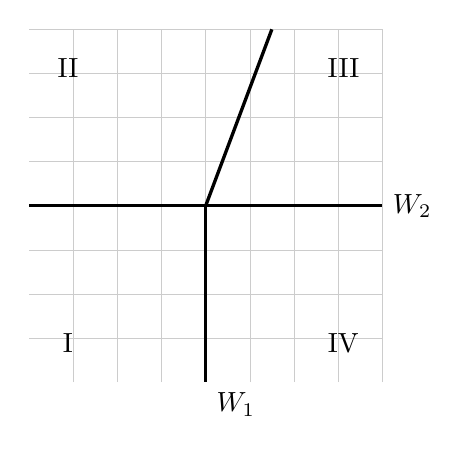
\begin{tikzpicture}[scale=0.7]

  % light square grid
  \draw[step=0.8cm,very thin,color=gray!40] (-3.2,-3.2) grid (3.2,3.2);

  % coordinate axes = walls
  \draw[very thick] (-3.2,0) -- (3.2,0) node[right] {$W_2$};
  \draw[very thick] (0,0) -- (0,-3.2) node[below right] {$W_1$};

  % slanted wall (ray) in quadrant III
  \draw[very thick] (0,0) -- (1.2,3.2);

  % chamber labels
  \node at (-2.5,-2.5) {$\mathrm{I}$};
  \node at (-2.5, 2.5) {$\mathrm{II}$};
  \node at ( 2.5, 2.5) {$\mathrm{III}$};
  \node at ( 2.5,-2.5) {$\mathrm{IV}$};

\end{tikzpicture}
\end{center}

\begin{itemize}
\item Let
\[
\cV = \cO_{\P^2_x\times\P^2_y}(-2,0)\oplus
      \cO_{\P^2_x\times\P^2_y}(-1,-3),
\]
and consider $\mathrm{tot}(\cV)$ as a toric variety given as a GIT
quotient of $\A^8$ by a torus $T\cong(\C^\ast)^2$ with weight matrix
$(t, s) \mapsto (t, t, t, s, s, s, t^{-2}, t^{-1}s^{-3})$.

\item One introduces a Landau-Ginzburg potential
\[
W = p f + q g \in \C[x_i,y_j,p,q]_{\deg=2},
\]
where $f$ has bidegree $(2,0)$ and $g$ has bidegree $(1,3)$, and $f$ cuts out a smooth rational curve on $\P^2_x$.
  The LG
pair $(\cV,W)$ carries a second $\C^\ast$–grading (the LG grading, "R-charge") so that the variables $p,q$ have weight
$2$ and the $x_i,y_j$ have weight $0$, so that $W$ has weight
$2$; the associated category $D^b(\cV,W)$ is equivalent to $D^b(X)$.

  The key point is that, although $Z_i/L_i$ is \emph{non-compact} as a
  usual GIT quotient, the restriction $W|_{Z_i}$ makes the LG quotient
  $(Z_i/L_i,W|_{Z_i})$ effectively compact.  Concretely:
  \begin{itemize}
  \item Near $W_1$ one has $Z_1/L_1 \cong \P^2/\C^\ast$; the LG
        category $D^b(Z_1/L_1,W|_{Z_1})$ is equivalent to
        $D^b(\P^2)$, which admits the full exceptional collection
        $\langle \cO,\cO(1),\cO(2)\rangle$.
  \item Near $W_2$ one has $Z_2/L_2 \cong \mathrm{tot}\,\cO_{\P^2}(-2)/\C^\ast$;
        the potential restricts to $pf$. Then
        $D^b(Z_2/L_2,W|_{Z_2})\simeq D^b(C)$, and for each window this is
        equivalent to $D^b(\P^1)$ with its exceptional pair
        $\langle\cO,\cO(1)\rangle$.
  \end{itemize}

\item One finds:
  \begin{itemize}
  \item the window shift across $W_1$ is a composition of spherical
        twists around the line bundles
        \[
        \cO_X(0,i),\ \cO_X(0,i+1),\ \cO_X(0,i+2),
        \]
  \item the window shift across $W_2$ is a composition of spherical
        twists around
        \[
        \cO_X(i,0),\ \cO_X(i+1,0),
        \]
  for suitable integers $i$ (depending on the chosen windows).
  \end{itemize}
\end{itemize}
\end{example}

\begin{thebibliography}{99}
\bibitem{HalpernLeistnerShipman2016}
D.~Halpern-Leistner and I.~Shipman, \emph{Autoequivalences of derived categories via geometric invariant theory}, 2016, arXiv:1303.5531. \url{https://arxiv.org/abs/1303.5531}.

\bibitem{Segal2011}
E.~Segal, \emph{Equivalences Between GIT Quotients of Landau-Ginzburg B-Models}, Comm. Math. Phys. \textbf{304} (2011), no.~2, 411--432. DOI:10.1007/s00220-011-1232-y.

\bibitem{SeidelThomas2000}
P.~Seidel and R.~P.~Thomas, \emph{Braid group actions on derived categories of coherent sheaves}, 2000, arXiv:math/0001043. \url{https://arxiv.org/abs/math/0001043}.

\end{thebibliography}

\end{document}